\section{Chapter 6. Electronic Structure of Atoms}

\secttoc

{\footnotesize
\begin{multicols}{3}
\begin{compactenum}
    \item Wavelength and frequency of electromagnetic radiation
    \item Order the common kinds of radiation according to wavelengths/energy
    \item Photons and their energy
    \item Line spectra, relate to quantized energy
    \item Wavelength of a moving object
    \item Uncertainty principle and what it limits
    \item Quantum numbers to the number and type of orbitals, orbital shapes
    \item Radial probability function graphs
    \item Hydrogen atom orbitals vs other atoms' orbitals
    \item Draw energy-level diagram for the orbitals in a many-electron
        atom, use Pauli exclusion principle and Hund's rule
    \item Using periodic table, write condensed electorn configurations. Number of unpaired $e^-$s.
\end{compactenum}
\end{multicols}
}

\begin{mdframed}
\subsection{Energy of Light and Photons, Quantum Worries}
\begin{multicols}{2}
\begin{compactdesc}
\item[Properties of light] speed of light $= c = 2.99 \cdot 10^8 \frac{m}{s} = \lambda \nu$
    where $\lambda$ is wave\textbf{l}ength $\nu$ is frequency.
\item[Energy of single photon] $E_p = h \nu$ where Planck's constant
    $h = 6.62E-43 J \cdot s$
\item[Wavelength of matter] $\lambda = h / mv$ related to mass and velocity.
\item[Heisenberg's uncertainty principle] $\Delta x \Delta (mv) \geq h / 4\pi$
    Position and momentum cannot be known perfectly.
\end{compactdesc}
\end{multicols}
\end{mdframed}




\begin{mdframed}
\begin{multicols}{2}
\subsection{Electron Orbitals}

\begin{figure}[H]
    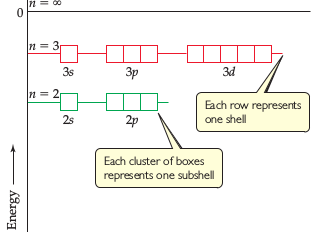
\includegraphics[width=0.4\textwidth]{electron_diagram.png}
\end{figure}
\begin{compactdesc}
\item[Electrons positioned] by using a probability distribution which depends on
    their energy level.
\item[Line spectrum]
\item[Spectral lines of Hydrogen] energy must be absorbed to emit an electron.
    Wavelength of each spectra line:
    \[
        \lambda = R_H(1/n_1^2 - 1/n_2^2)
    \]
\item[Energy of hydrogen emissions]
    \[
        \Delta E = -2.18*10^{-18}J \big(1/n_f^2 -n_i^2 \big)
    \]
\item[Orbital diagram] visualization of each $e^-$'s quantum numbers in an
    atom or molecule. Row of boxes, one box holds at most a pair of arrows
    pointing in opposite directions ($e^-$) and groups of boxes are slightly
    separated to indicate different orbitals p, s, d, f.
\item[Electron Quantum Numbers] $n, l, m_l, m_s$
\item[Energy level] $n \in N^+$
\item[Orbitals] p, s, d, f $l \in 0\dots n - 1$
\item[Magnetic quantum number] a box, $m_s \in -l \dots l$
\item[Spin magnetic quantum number] up/down, $m_l = \pm 1/2$
\item[Subshell] electrons share $n, l$
\item[Pauli's exclusion principle] all $e^-$ in an atom have unique quantum
    numbers.
\item[Hund's rule] the preferred $e^-$ arrangement has maximum $e^-$ with the
    same spin $m_s$
\end{compactdesc}

\begin{figure}[H]
    \centering
    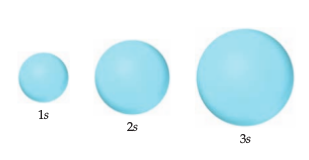
\includegraphics[width=0.2\textwidth]{s_orbital.png}
    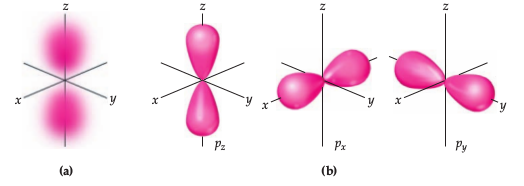
\includegraphics[width=0.3\textwidth]{p_orbitals.png}
    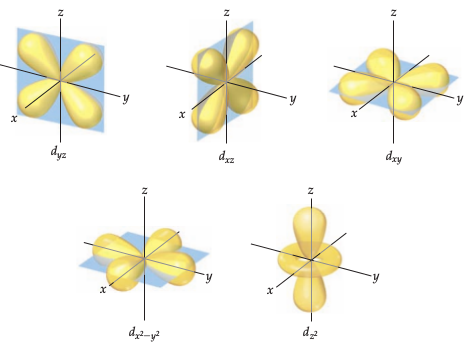
\includegraphics[width=0.3\textwidth]{d_orbitals.png}
\end{figure}

\end{multicols}
\end{mdframed}



